\section{Results for Atoms}
 
 \subsection{Ground State Energies}
 
\begin{table}
\begin{center}
\caption{Ground state energies for Atoms calculated using Variational - and Diffusion Monte-Carlo. Experimental energies are listed in the last column. As we see, DMC is rather close to the experimental energy. $\epsilon_\mathrm{rel} = |E_\mathrm{DMC} - \mathrm{Expt.}|/|\mathrm{Expt.}|$}
\begin{tabular}{lp{2cm}cclc}
Atom & & $E_\mathrm{VMC}$ & \qquad $E_\mathrm{DMC}$ & \qquad\,\, Expt. & \qquad $\epsilon_\mathrm{rel}$\\
\hline\hline
\ \\
He & \qquad & -2.8903(2) & \qquad -2.9036(2) & \qquad $-2.9037^\mathrm{a}$ & \qquad $3.44\cdot 10^{-5}$\\
\ \\
Be & \qquad & -14.145(2) & \qquad -14.657(2)  & \qquad $-14.6674^\mathrm{a}$ & \qquad $7.10\cdot 10^{-4}$ \\
\ \\
Ne & \qquad & -127.853(2) & \qquad -128.765(4) & \qquad $-128.9383^\mathrm{a}$ & \qquad $1.34\cdot 10^{-3}$  \\
\ \\
Mg & \qquad & -197.269(3) & \qquad -199.904(8) & \qquad $-200.054^\mathrm{a}$ & \qquad $7.50\cdot 10^{-4}$  \\
\ \\
Ar & \qquad & -524.16(7) & \qquad -527.30(4) & \qquad $-527.544^\mathrm{a}$ & \qquad $4.63\cdot 10^{-4}$  \\
\ \\
Kr & \qquad & -2700(5) & \qquad -2749.9(2) & \qquad $-2752.05498^\mathrm{b}$ & \qquad $7.83\cdot 10^{-4}$  \\
\ \\
\end{tabular}
\label{tab:AtomsRes}
\end{center}
\end{table}
 
 
 \subsection{The Noble-Gases}
 
 blah blah
 
 nuclear interaction extremely dominating. One-body densities utterly boring; exponential decay from core.
 
 Interesting still: angular averaged radial one-body density.

 More dispersed = More chemically unstable. 
 
 As expected Krypton is most stable.
 
 
\begin{figure}
 \begin{center}
   \subfigure{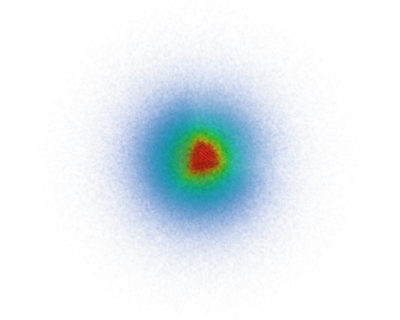
\includegraphics[scale=0.46]{../Graphics/OBD/OBD_Atoms/3D/Helium.png}} 
   \subfigure{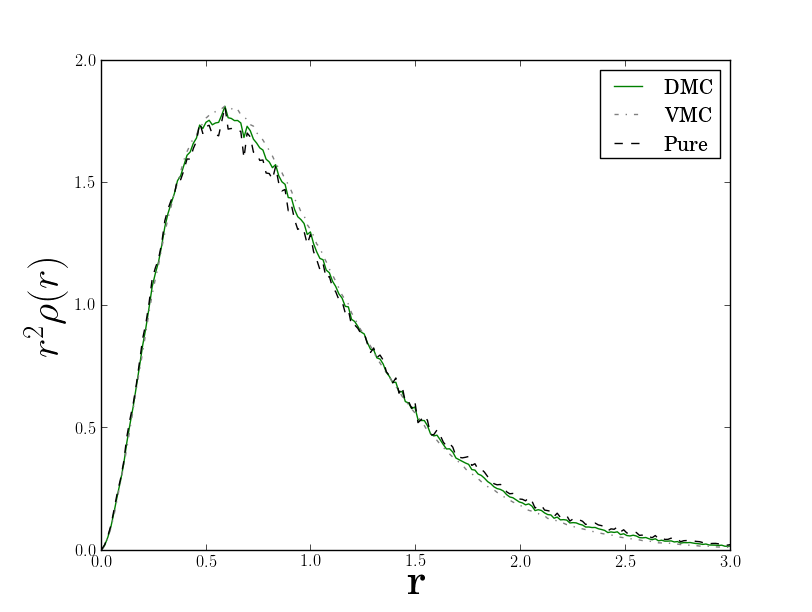
\includegraphics[scale=0.33]{../Graphics/OBD/OBD_Atoms/2D/Helium.png}}  \\
   \subfigure{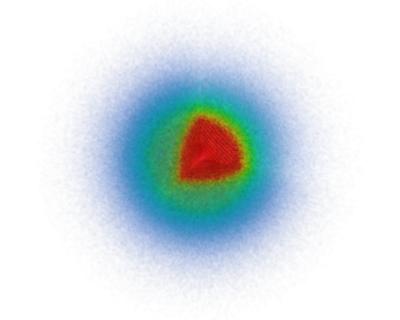
\includegraphics[scale=0.46]{../Graphics/OBD/OBD_Atoms/3D/Neon.png}} 
   \subfigure{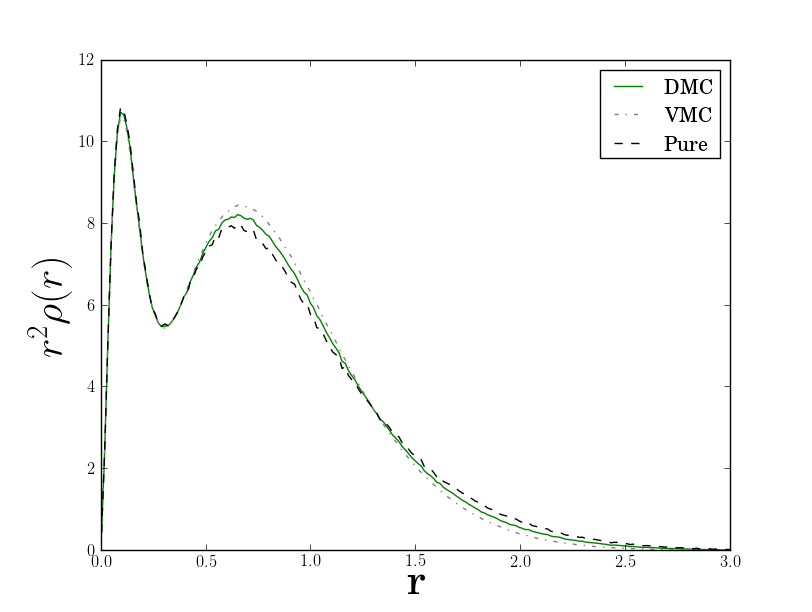
\includegraphics[scale=0.33]{../Graphics/OBD/OBD_Atoms/2D/Neon.png}}  \\
   \subfigure{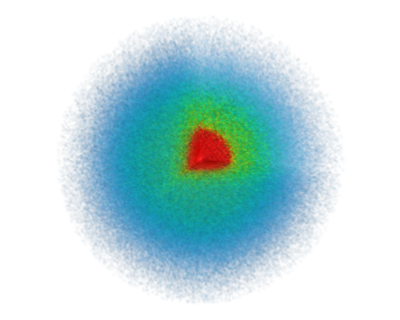
\includegraphics[scale=0.46]{../Graphics/OBD/OBD_Atoms/3D/Argon.png}} 
   \subfigure{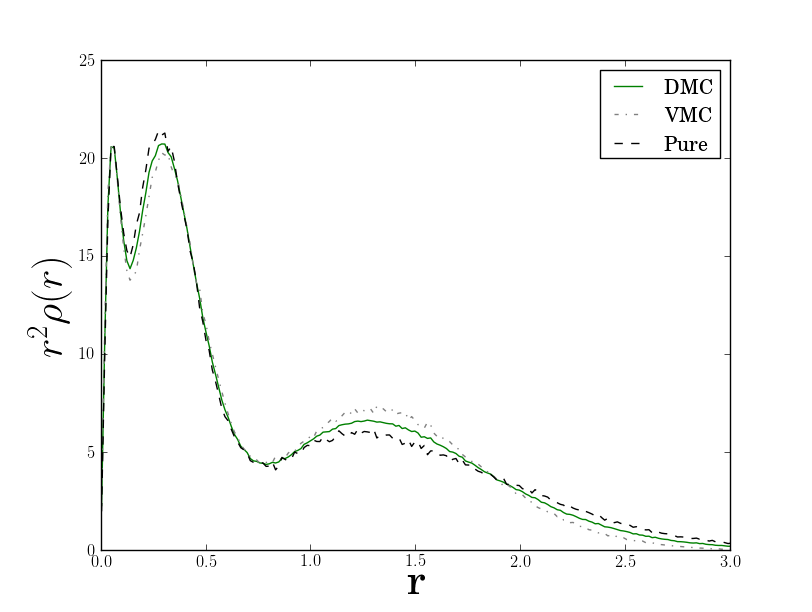
\includegraphics[scale=0.33]{../Graphics/OBD/OBD_Atoms/2D/Argon.png}}  \\
   \subfigure{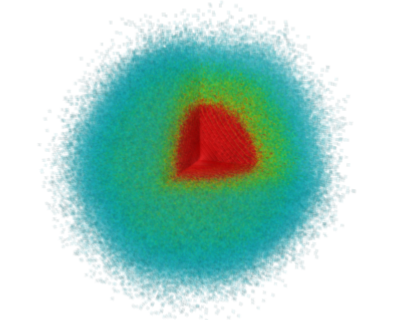
\includegraphics[scale=0.46]{../Graphics/OBD/OBD_Atoms/3D/Krypton.png}} 
   \subfigure{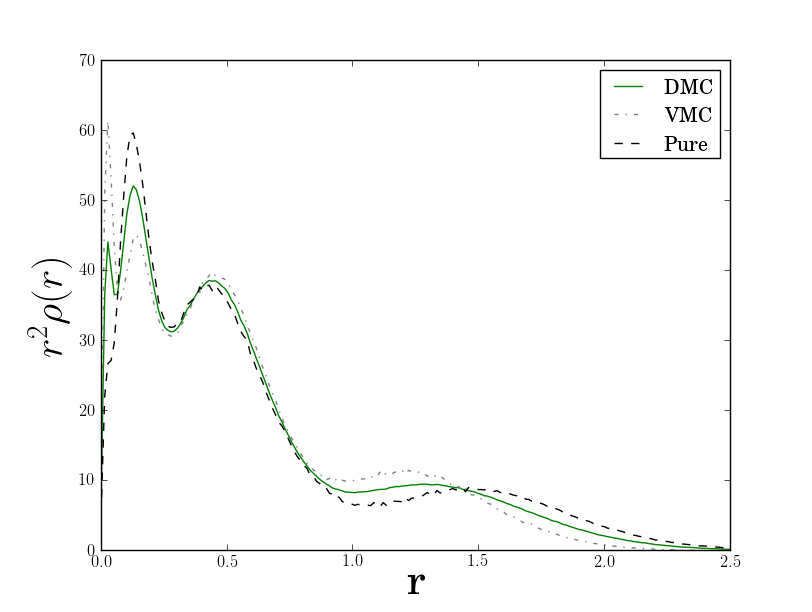
\includegraphics[scale=0.33]{../Graphics/OBD/OBD_Atoms/2D/Krypton.png}}  \\
  \caption{Counting top to bottom: Helium, Neon, Argon and Krypton. See Fig. \ref{fig:OBD_alkaline_Atoms_2D_combo} for descriptions.}
  \label{fig:OBD_noble_Atoms_2D_combo}
 \end{center}
\end{figure}

 
 \clearpage
 
 
 \subsection{Alkaline Earth Metals}
 
 blah blah good approximation with one determinant -> calculations possible. 
 
 More smushed out; missing contribution from higher |m| since the shell is not closed. 
 
 DMC still are able to span out a more correct wave function. This is backed up by experimental data comparisons. 
 
 The densities are similar to their close noble-gas relative, however, the two additional particles creates a disperse probability cloud. The noble gases have more well-defined (sharp) shell structures.
 
 Another interesting fact: VMC distribution and the estimated pure DMC distribution is more different for the alkaline earth metals than for the noble gases. This is expected since M=0 S=0 ground state is major contributions from 3p 2p states. 
 
 
\begin{figure}
 \begin{center}
   \subfigure{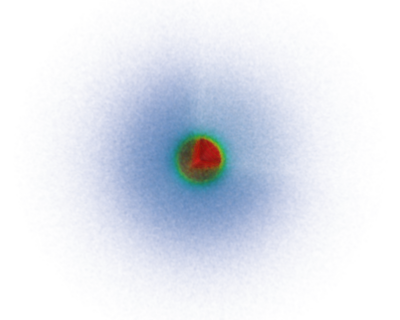
\includegraphics[scale=0.5]{../Graphics/OBD/OBD_Atoms/3D/Beryllium.png}} 
   \subfigure{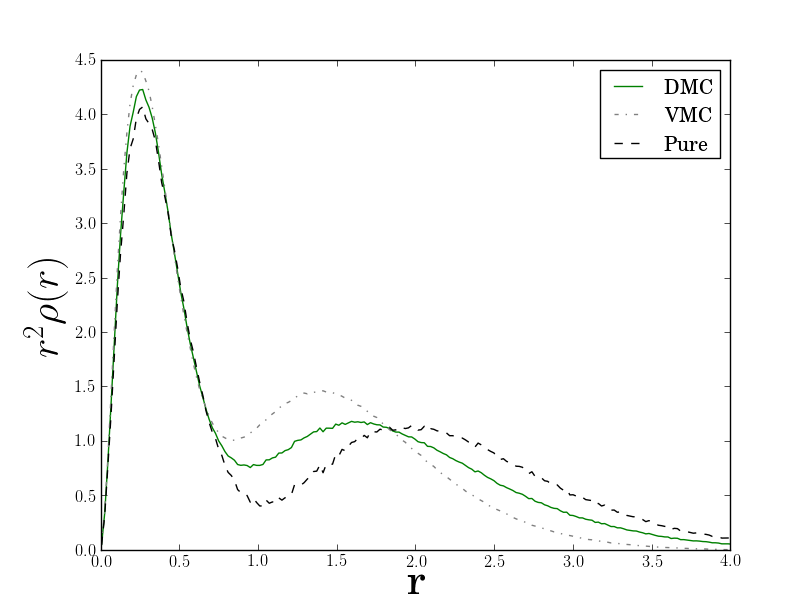
\includegraphics[scale=0.38]{../Graphics/OBD/OBD_Atoms/2D/Beryllium.png}}  \\
   \subfigure{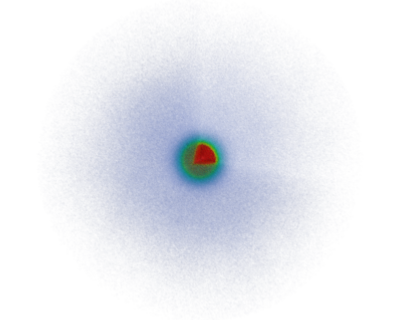
\includegraphics[scale=0.5]{../Graphics/OBD/OBD_Atoms/3D/Magnesium.png}} 
   \subfigure{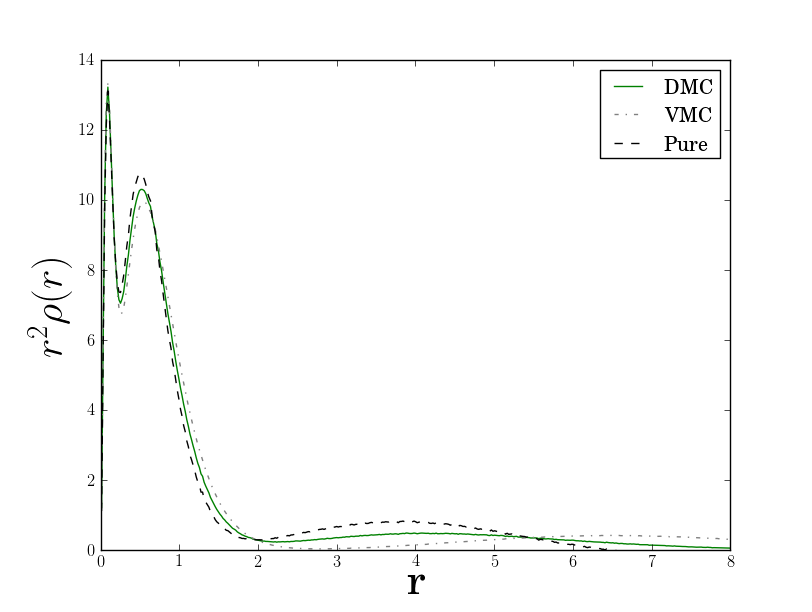
\includegraphics[scale=0.38]{../Graphics/OBD/OBD_Atoms/2D/Magnesium.png}}  \\
   \vspace{0.5cm}
   \subfigure{
\includegraphics[scale=1.5]{../Graphics/OBD/OBD_Atoms/3D/colorbar.png}}
   \vspace{0.5cm}
  \caption{Three dimensional one-body density (left column) and angular averaged radii (right column) for alkaline earth metals; Beryllium (top) and Magnesium (bottom). The color bar shows increasing values from left to right. Notice that it is not the radial one-body density (which is too steep to reveal characteristics) in the right column, but the electron . Compared to the noble gases in Fig.~\ref{fig:OBD_noble_Atoms_2D_combo}, the alkaline earth metals have a surrounding dispersed probability cloud due to the broken closed shell symmetry. The element is thus more unstable and potent for chemical reactions and molecular formations through covalent bonds.}
  \label{fig:OBD_alkaline_Atoms_2D_combo}
 \end{center}
\end{figure}